% Asset ID: FAS2RecurrenceRelationshipsTikZ-001
% Source: Uploaded recurrence relations transcript, staircase-counting example.
% Related lesson section: # 9. Visual Asset Integration and # 11. Worked Examples
% Used placeholder:
% [VISUAL PLACEHOLDER: FAS2RecurrenceRelationshipsTikZ-001 | Source: Uploaded transcript staircase-counting example | Insert from tikz/FAS2RecurrenceRelationshipsTikZ-001.tex | Purpose: Show why S_n=S_{n-1}+S_{n-2} by splitting according to Claudia’s first step.]
% Purpose: Show why S_n = S_{n-1} + S_{n-2} by splitting the staircase problem according to the first move.
% Creation notes:
% This diagram represents the transcript logic:
% If Claudia first takes 1 step, there are n - 1 steps left, giving S_{n-1} completions.
% If Claudia first takes 2 steps, there are n - 2 steps left, giving S_{n-2} completions.
% These two cases are exhaustive and non-overlapping, so S_n = S_{n-1} + S_{n-2}.

\documentclass[tikz,border=8pt]{standalone}

\usepackage{amsmath}
\usepackage{xcolor}
\usetikzlibrary{arrows.meta,positioning,calc,decorations.pathreplacing}

\definecolor{Canvas}{HTML}{FAF9F6}
\definecolor{Ivory}{HTML}{FFFFF0}
\definecolor{Line}{HTML}{E5E5EA}
\definecolor{Gold}{HTML}{C5A059}
\definecolor{DeepGold}{HTML}{D4AF37}
\definecolor{SoftPink}{HTML}{FBEFEF}
\definecolor{Text}{HTML}{2C2C2E}

\begin{document}

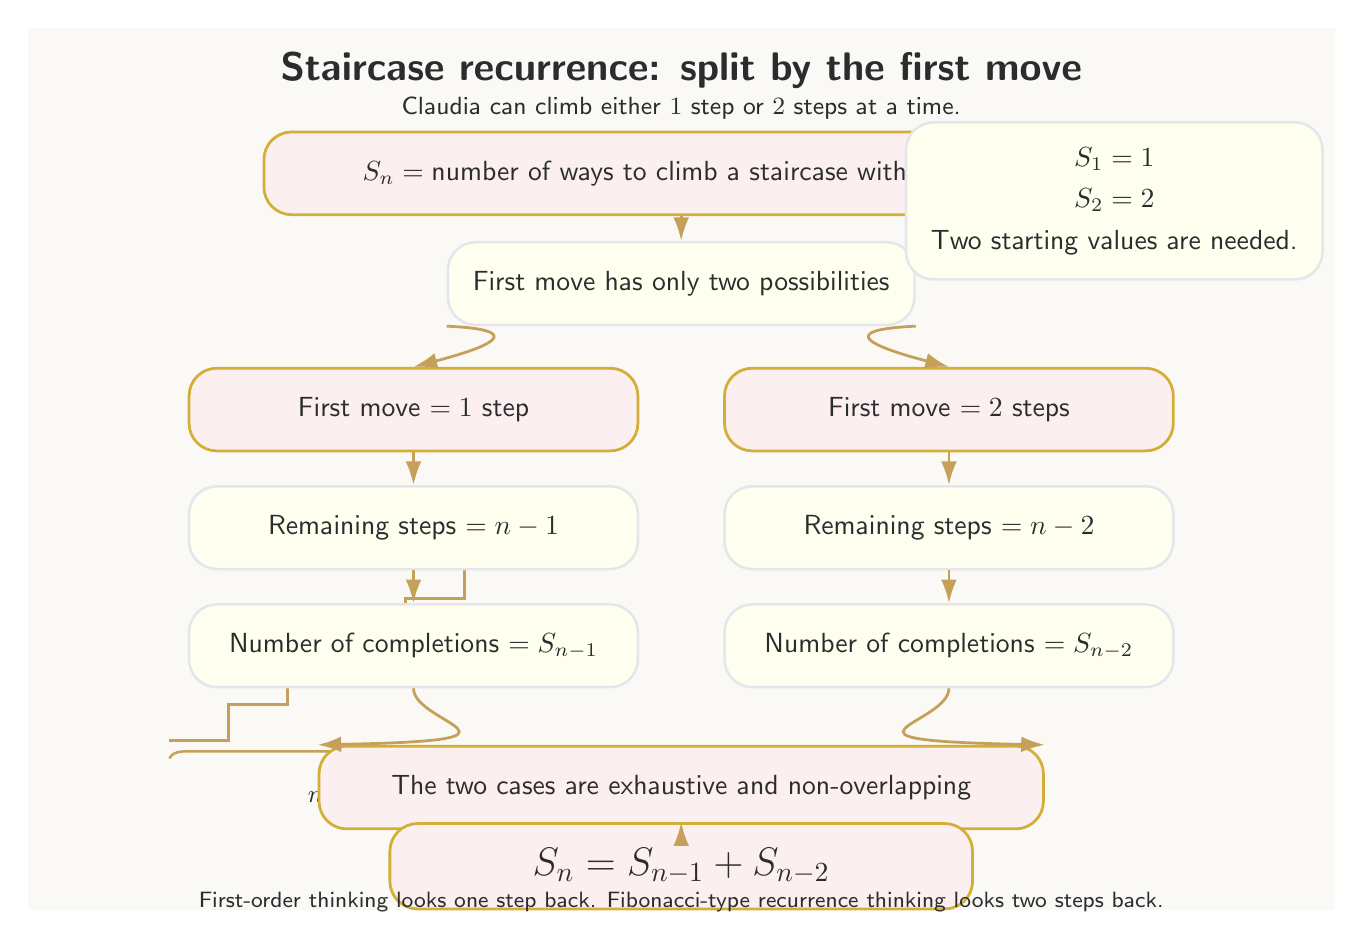
\begin{tikzpicture}[
    font=\sffamily,
    text=Text,
    box/.style={
        rounded corners=10pt,
        draw=Line,
        line width=0.9pt,
        fill=Ivory,
        align=center,
        inner sep=9pt,
        minimum height=1.05cm
    },
    highlight/.style={
        rounded corners=10pt,
        draw=DeepGold,
        line width=1pt,
        fill=SoftPink,
        align=center,
        inner sep=9pt,
        minimum height=1.05cm
    },
    arrow/.style={
        -{Latex[length=3mm,width=2mm]},
        line width=1pt,
        draw=Gold
    },
    stair/.style={
        draw=Gold,
        line width=1pt
    },
    labeltext/.style={
        font=\sffamily\small,
        text=Text,
        align=center
    },
    mathtext/.style={
        font=\sffamily\large,
        text=Text,
        align=center
    }
]

% Background
\fill[Canvas] (-0.8,-5.0) rectangle (15.8,6.2);

% Title
\node[font=\sffamily\bfseries\Large, text=Text] at (7.5,5.65)
{Staircase recurrence: split by the first move};

\node[font=\sffamily\small, text=Text, align=center] at (7.5,5.18)
{Claudia can climb either \(1\) step or \(2\) steps at a time.};

% Main definition box
\node[highlight, minimum width=10.6cm] (def) at (7.5,4.35)
{\(\displaystyle S_n=\text{number of ways to climb a staircase with }n\text{ steps}\)};

% Staircase drawing
\coordinate (A) at (1.0,-2.85);
\draw[stair] (A) -- ++(0.75,0) -- ++(0,0.45) -- ++(0.75,0) -- ++(0,0.45)
             -- ++(0.75,0) -- ++(0,0.45) -- ++(0.75,0) -- ++(0,0.45)
             -- ++(0.75,0) -- ++(0,0.45) -- ++(0.75,0) -- ++(0,0.45)
             -- ++(0.75,0);

\node[labeltext] at (3.6,0.15) {A staircase with \(n\) steps};

\draw[decorate, decoration={brace, amplitude=5pt}, draw=Gold, line width=0.9pt]
(1.0,-3.08) -- (5.5,-3.08)
node[midway, below=7pt, labeltext] {\(n\) steps};

% Decision box
\node[box, minimum width=5.6cm] (decision) at (7.5,2.95)
{First move has only two possibilities};

\draw[arrow] (def.south) -- (decision.north);

% Branch boxes
\node[highlight, minimum width=5.7cm] (one) at (4.1,1.35)
{First move \(=1\) step};

\node[highlight, minimum width=5.7cm] (two) at (10.9,1.35)
{First move \(=2\) steps};

\draw[arrow] (decision.south west) .. controls (5.8,2.35) and (4.7,2.05) .. (one.north);
\draw[arrow] (decision.south east) .. controls (9.2,2.35) and (10.3,2.05) .. (two.north);

% Consequence boxes
\node[box, minimum width=5.7cm] (oneleft) at (4.1,-0.15)
{Remaining steps \(=n-1\)};

\node[box, minimum width=5.7cm] (twoleft) at (10.9,-0.15)
{Remaining steps \(=n-2\)};

\draw[arrow] (one.south) -- (oneleft.north);
\draw[arrow] (two.south) -- (twoleft.north);

\node[box, minimum width=5.7cm] (oneways) at (4.1,-1.65)
{Number of completions \(=S_{n-1}\)};

\node[box, minimum width=5.7cm] (twoways) at (10.9,-1.65)
{Number of completions \(=S_{n-2}\)};

\draw[arrow] (oneleft.south) -- (oneways.north);
\draw[arrow] (twoleft.south) -- (twoways.north);

% Combine
\node[highlight, minimum width=9.2cm] (combine) at (7.5,-3.45)
{The two cases are exhaustive and non-overlapping};

\draw[arrow] (oneways.south) .. controls (4.1,-2.65) and (5.9,-2.85) .. (combine.north west);
\draw[arrow] (twoways.south) .. controls (10.9,-2.65) and (9.1,-2.85) .. (combine.north east);

\node[highlight, minimum width=7.4cm, font=\sffamily\Large] (result) at (7.5,-4.45)
{\(\displaystyle S_n=S_{n-1}+S_{n-2}\)};

\draw[arrow] (combine.south) -- (result.north);

% Initial conditions note
\node[box, minimum width=4.8cm, align=center] at (13.0,4.0)
{\(\displaystyle S_1=1\)\\[3pt]
\(\displaystyle S_2=2\)\\[3pt]
Two starting values are needed.};

% Footer note
\node[font=\sffamily\footnotesize, text=Text, align=center] at (7.5,-4.9)
{First-order thinking looks one step back. Fibonacci-type recurrence thinking looks two steps back.};

\end{tikzpicture}

\end{document}
